\documentclass[conference]{IEEEtran}
\usepackage{cite}
\usepackage{amsmath,amssymb,amsfonts}
\usepackage{algorithmic}
\usepackage{graphicx}
\usepackage{textcomp}
\usepackage{xcolor}
\usepackage{svg}
\def\BibTeX{{\rm B\kern-.05em{\sc i\kern-.025em b}\kern-.08em
    T\kern-.1667em\lower.7ex\hbox{E}\kern-.125emX}}
    
\title{LEPL1110 - Introduction aux éléments finis
 \\ {\huge Projet 1}}
\author{
\IEEEauthorblockN{Pierre Leboutte}
\IEEEauthorblockA{\textit{4330-21-00} \\}

\IEEEauthorblockN{Giovanni Karra}
\IEEEauthorblockA{\textit{4503-21-00} \\}
}

\begin{document}
\maketitle

\section*{Physique du problème}
Notre problème consiste en la torsion des rayons d'une roue de vélo, modélisée comme un moyen central et une couronne extérieure reliée par des rayons, soumise à des forces de freinage. \\
Notons les conditions suivantes:
\begin{itemize}
    \item Moyeu central : conditions de Dirichlet en X Y pour modéliser l'encastrement.
    \item Couronne extérieure : condition de Neumann, avec une force tangentielle appliquée sur la couronne pour représenter le moment de freinage.
\end{itemize}
Notons qu'il est possible de faire varier un certain nombre de paramètre(largeur de la roue, nombre de rayons...)
\begin{figure}[h]
    \centering
    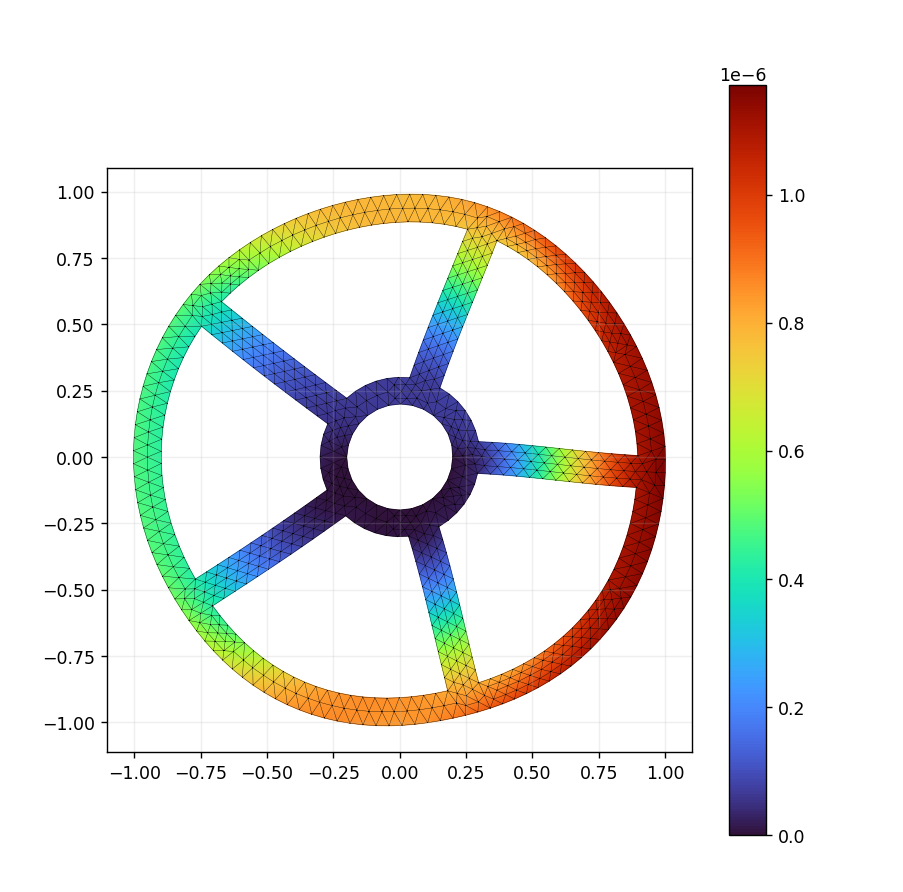
\includegraphics[width=0.5\textwidth]{../Figures/roue.png}
    \caption{Animation de notre roue}
\end{figure}


\section*{Quid en théorie...}
En assimilant chaque rayon à une poutre en torsion encastrée à ses deux extrémités, de longueur $L$ et de section circulaire de rayon $R$, on peut calculer analytiquement la rotation $\theta$ de la jante par rapport au moyeu sous l'effet d'un couple $C$ :
\begin{equation}
\theta = \frac{CL}{n\pi R^4 G}
\end{equation}
où $n$ est le nombre de rayons et $G$ le module de cisaillement du matériau. La contrainte de cisaillement maximale dans les rayons vaut alors :
\begin{equation}
\tau_\text{max} = \frac{CR}{n\pi R^4} = \frac{C}{n\pi R^3}
\end{equation}
Nous avons pu vérifier que ces valeurs calculées se rapprochent des valeurs observées en pratique. 

\section*{... et en pratique?}
Après avoir généré notre maillage, nous solvons notre matrice à l'aide d'un \textbf{solveur bande}. \\
Comme vu au cours, nous savons que dans une matrice creuse comme celle-ci, il est possible de considérablement réduire le nombre d'opérations effectuées, comme la consommation de mémoire. Nous utilisons une renumérotation qui permute les lignes et colonnes de la matrice, de manière à réduire considérablement notre bande, et gagner ainsi du temps lors du solving. \\
Nous avons également envisagé un renumérotation du type Reverse Cuthill-McKee, mais par manque de temps nous avons utilisé uniquement une renumérotation selon la coordonnée Y, ce qui donne déjà de très bons résultats.
\begin{figure}[h]
    \centering
    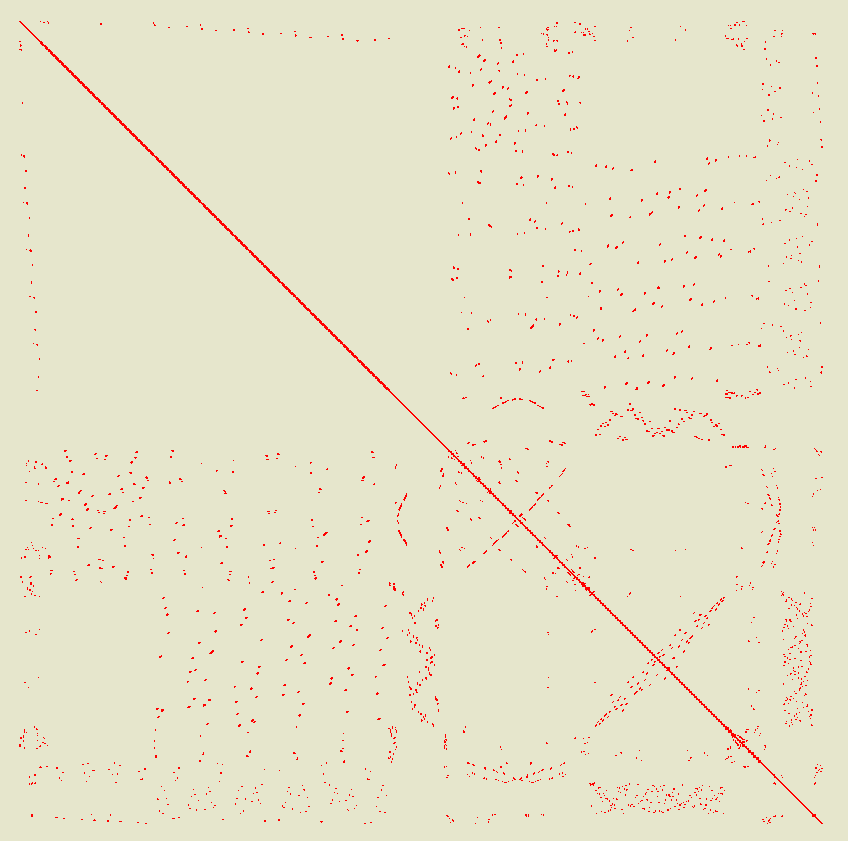
\includegraphics[width=0.2\textwidth]{../Figures/sans_renum.png}
    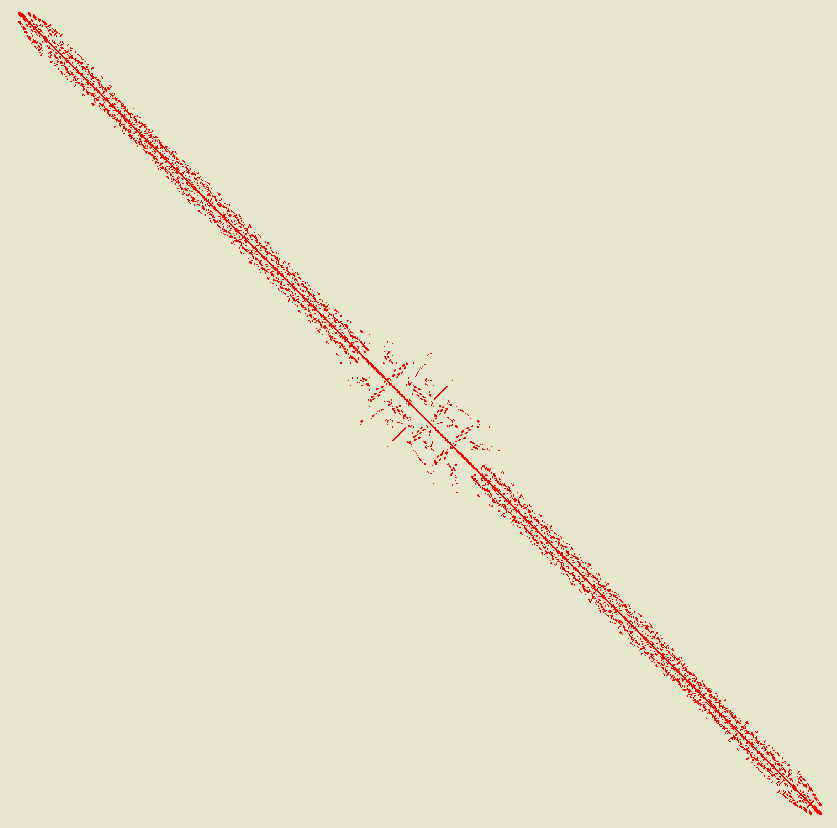
\includegraphics[width=0.2\textwidth]{../Figures/avec_renum.png}
    \caption{Effet de la renumérotation}
\end{figure}

\section*{Analyse des résultats obtenus}

En faisant varier les paramètres correspondants, nous avons relevé les observations suivantes: 
\begin{itemize}
    \item Lorsque l'épaisseur des rayons augmente (c'est à dire leur rigidité), la déformation en torsion diminue
    \item Lorsque le nombre de rayons augmente, la déformation en torsion diminue également, car la répartition des efforts est mieux répartie sur l'ensemble de la roue.
    \item Les contraintes maximales sont observées aux jonctions entre le moyeu central et les rayons, également entre les rayons et la couronne extérieur. 
\end{itemize}


\section*{Performances}
Nous apouvons observer sur le graphe (en log-log) suivant que les performances suivent une loi exponentielle en $\mathcal{O}(h^3)$
\begin{figure}[h]
    \centering
    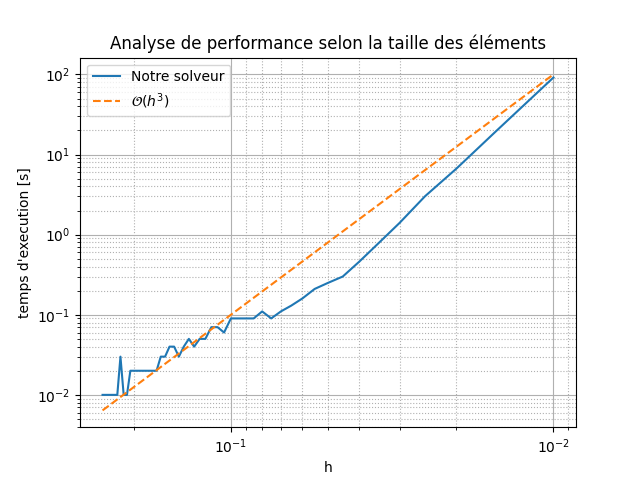
\includegraphics[width=0.5\textwidth]{../Figures/perf.png}
    \caption{Analyse de performance}
\end{figure}


\section*{Transition}
Dans l'optique de mise en avant des moyens de transport "propres", nous avons jugé pertinent pour l'avenir de rechercher des manières de concevoir les freins, la roue et les rayons avec des composants durables. Cela nous a éclairé sur la nécessité d'utiliser du \textbf{caoutchouc} pour les freins et le pneu, au vu de son coefficient de poisson plus élevé qui évite ainsi les déformations. Cyclistes nous-mêmes, nous avons pu nous rendre compte que les freins sont parmi les composants les plus usés en moyenne, et il nous paraissait judicieux de nous pencher sur cette question pour des questions de sécurité, économiques et écologiques
\section*{Animation}
Nous avons mis au point une simulation, disponible au QR code suivant, qui illustre la déformation obtenue par en exerçant une force tangentielle de plus en plus grande. La force va de de 16N à 1000N.
\begin{figure}[h]
    \centering
    
\includegraphics[width=0.3\textwidth]{../Figures/QR.png}
    \caption{Animation de notre roue}
\end{figure}

\section*{Conclusion}
En guise de conclusion, permettons-nous de rappeler que le travail constitue une base extensible, via l'utilisation souhaitable de différents coefficients de Poisson propre à chaque élément du système (roue, jante, moyeu central) et l'ajout de composants - comme le pneu - permettant d'enrichir davantage le modèle.

\section*{Références}
\begin{enumerate}
    \item L.N. Trefethen et D. Bau. Numerical Linear Algebra. Siam, 1997.
\end{enumerate}
\end{document}